% k=2/3 and P=(13/4,5/6); the labels give the general equations.
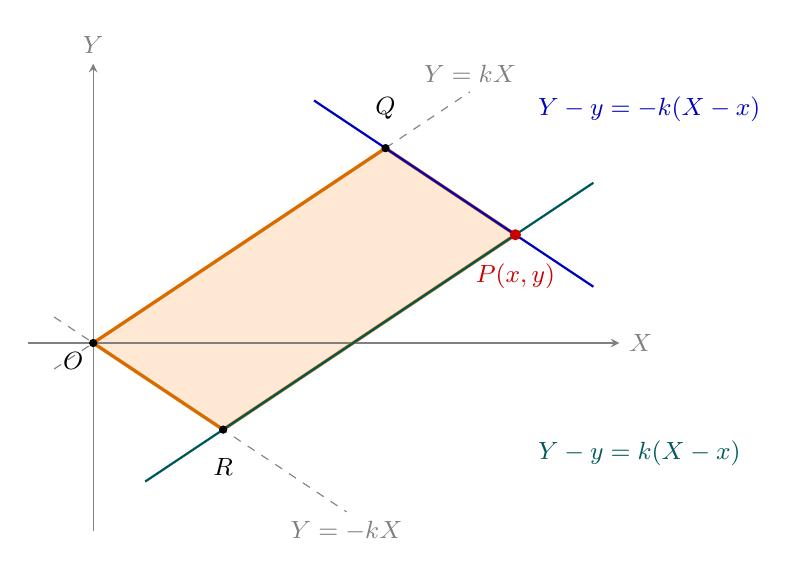
\begin{tikzpicture}[x=1.65cm,y=1.65cm,>=stealth,font=\small]
\coordinate (O) at (0,0); \coordinate (Q) at (2.25,1.5);
\coordinate (R) at (1,-2/3); \coordinate (P) at (3.25,5/6);
\fill[orange!17] (O)--(Q)--(P)--(R)--cycle;
\draw[->,gray] (-.5,0)--(4.05,0) node[right] {$X$};
\draw[->,gray] (0,-1.45)--(0,2.15) node[above] {$Y$};
\draw[gray,dashed] (-.3,-.2)--(2.9,29/15) node[above] {$Y=kX$};
\draw[gray,dashed] (-.3,.2)--(1.95,-1.3) node[below] {$Y=-kX$};
\draw[orange!85!black,very thick] (O)--(Q)--(P)--(R)--cycle;
\draw[blue!75!black,thick] (1.7,28/15)--(3.85,13/30);
\draw[teal!70!black,thick] (.4,-16/15)--(3.85,37/30);
\node[anchor=west,blue!75!black] at (3.35,1.8) {$Y-y=-k(X-x)$};
\node[anchor=west,teal!70!black] at (3.35,-.85) {$Y-y=k(X-x)$};
\fill (O) circle(1.5pt) node[below left] {$O$};
\fill (Q) circle(1.5pt) node[above=7pt] {$Q$};
\fill (R) circle(1.5pt) node[below=7pt] {$R$};
\fill[red!80!black] (P) circle(2pt) node[below=7pt] {$P(x,y)$};
\end{tikzpicture}
